% chapter2.tex

\chapter{Simple Clouds Model}  
\label{ch:chapter2}


In this chapter, the literature about clouds and cloud schemes will be reviewed. The roles of clouds in climate system is reviewed in Section \ref{sec:chp2_role_of_clouds}. A brief history of cloud scheme development is reviewed in  \ref{sec:chp2_cld_scheme}

%\epigraph{\textit{Let's begin the scientific journey!}}{\textit{Qun Liu}, 2018}

\section{Roles of clouds in climate system}
\label{sec:chp2_role_of_clouds}
% Literature review about the role of clouds in climate system

Clouds usually cover more than half areas of the Earth at any given time \citep{Houze2014} and play a fundamental role in Earth's radiation budget and hydrological cycle. In general, clouds can reflect the sunlight (shortwave radiation) back into space and absorb the longwave radiation emitted from the surface, part of which will return to the surface. In general, the net effect of cloud is to cool the earth comparing to the cloud-free conditions. According to \cite{Zelinka2017}, the net cooling effect of clouds is about 18 Wm$^{-2}$, which is roughly five times as large as the heating effect of doubling CO$_2$. Therefore, even a small change of clouds could have large influence to the climate, that's one possible reason that why the cloud feedback is so important in climate system. \\


Cloud feedback is the variation of cloud radiative forcing at top-of-atmosphere (TOA) in response to global warming. In the fifth assessment report of the Intergovernmental Panel on Climate Change (IPCC AR5), the sign of net cloud radiative feedback is likely positive with an estimate of 0.6 Wm$^{-2}$K$^{-1}$ \citep{stocker2013climate}, which, however, has a lot of uncertainties. As shown in Figure \ref{fig:cld_feed_back_ecs}, comparing to the water vapor, lapse rate and albedo feedbacks, cloud feedback have the largest spread, which in fact is the largest uncertainty of simulated climate response to CO$_2$ foricng (i.e. climate sensitivity) in the general circulation models (GCMs) \citep{Ceppi2017}. Lots of efforts have been payed to investigate the possible reasons for the uncertainty of cloud feedbacks. For example, \cite{Webb2015} has proposed the Selected Process On/Off Klima Intercomparison Experiment (SPOOKIE) project, where the role of the convection has been accessed in the first phase of the project. They conclude that while parametrized convection influences the strength of the cloud feedbacks substantially in some models, other processes must also contribute substantially to the overall inter-model spread. In the second phase, the roles of cloud scheme will be examined. %, where the cloud fraction, cloud water content and effective cloud droplets radius are prescribed or will be diagnosed empirically.


\begin{figure}[h]
	\centering
	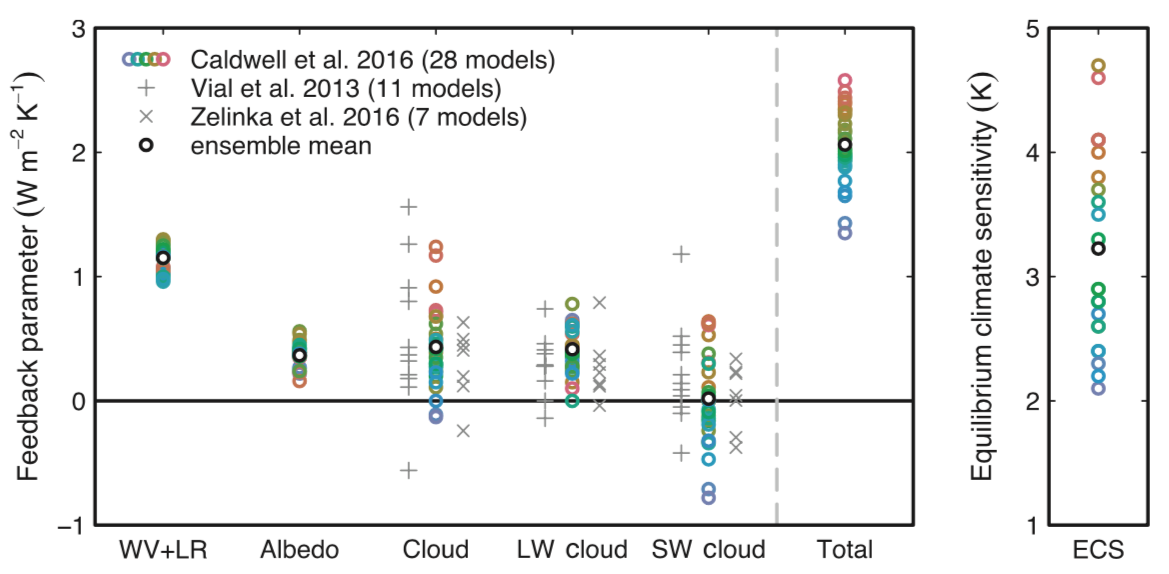
\includegraphics[width=1\linewidth]{{figs/chp2/cloud_feedback_ceppi}.png}
	\caption{Strengths of individual global-mean feedbacks and equilibrium climate sensitivity (ECS) for CMIP5 models, derived from coupled experiments with abrupt quadrupling of CO$_2$ concentration. Circles are colored according to the total feedback parameter. The Planck feedback (mean value of -3.15 W m$^{-2}$ K$^{-1}$) is excluded from the total feedback parameter shown here. Adapted from \cite{Ceppi2017}.}
	\label{fig:cld_feed_back_ecs}
\end{figure}

%\section{Cloud Radiative Effect and its feedback}

%\section{Method: Diagnosis of cloud}
\section{Cloud schemes}
\label{sec:chp2_cld_scheme}

